\begin{center}
\tikzset{every picture/.style={line width=0.75pt}} %set default line width to 0.75pt        

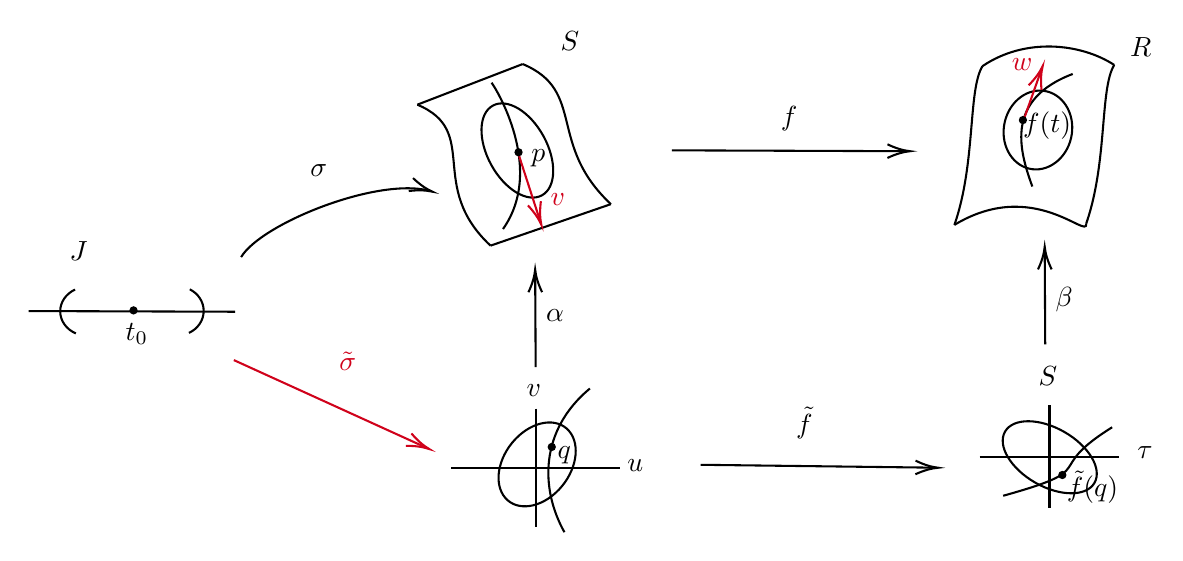
\begin{tikzpicture}[x=0.75pt,y=0.75pt,yscale=-1,xscale=1]
%uncomment if require: \path (0,300); %set diagram left start at 0, and has height of 300

%Shape: Ellipse [id:dp2910737338157192] 
\draw   (298.08,209.7) .. controls (303.85,216.44) and (301.65,229.11) .. (293.16,238.01) .. controls (284.67,246.9) and (273.11,248.65) .. (267.33,241.91) .. controls (261.56,235.17) and (263.76,222.49) .. (272.25,213.6) .. controls (280.74,204.71) and (292.3,202.96) .. (298.08,209.7) -- cycle ;
%Curve Lines [id:da929254968628841] 
\draw    (295.87,258.5) .. controls (284.07,237.43) and (283.92,209.33) .. (308.12,189.26) ;
\draw   (241.25,227.39) -- (322.64,227.39)(281.95,198.96) -- (281.95,255.82) ;
%Shape: Free Drawing [id:dp8489877677824506] 
\draw  [line width=3] [line join = round][line cap = round] (289.75,217.42) .. controls (289.75,217.42) and (289.75,217.42) .. (289.75,217.42) ;
%Straight Lines [id:da862614773060371] 
\draw    (282,179) -- (281.76,133.92) ;
\draw [shift={(281.75,131.92)}, rotate = 89.7] [color={rgb, 255:red, 0; green, 0; blue, 0 }  ][line width=0.75]    (10.93,-3.29) .. controls (6.95,-1.4) and (3.31,-0.3) .. (0,0) .. controls (3.31,0.3) and (6.95,1.4) .. (10.93,3.29)   ;
%Straight Lines [id:da3359096313011646] 
\draw    (225,52.5) -- (275.75,32.92) ;
%Curve Lines [id:da3343463368770112] 
\draw    (225,52.5) .. controls (255.75,65.42) and (229.25,91.42) .. (260.25,120.42) ;
%Curve Lines [id:da48380373492309947] 
\draw    (275.75,32.92) .. controls (306.5,45.83) and (287.25,71.42) .. (318.25,100.42) ;
%Straight Lines [id:da8917905611546483] 
\draw    (260.25,120.42) -- (318.25,100.42) ;
%Shape: Ellipse [id:dp6506547988207897] 
\draw   (261.35,52.96) .. controls (268.31,49.15) and (279.24,55.74) .. (285.77,67.68) .. controls (292.3,79.62) and (291.96,92.38) .. (285,96.19) .. controls (278.04,100) and (267.11,93.4) .. (260.58,81.46) .. controls (254.05,69.53) and (254.39,56.76) .. (261.35,52.96) -- cycle ;
%Curve Lines [id:da04665611580793161] 
\draw    (266.25,112.42) .. controls (286.75,83.42) and (262.75,44.42) .. (260.75,41.92) ;
%Straight Lines [id:da39496589729408993] 
\draw [color={rgb, 255:red, 208; green, 2; blue, 27 }  ,draw opacity=1 ]   (273.17,74.57) -- (284.14,108.51) ;
\draw [shift={(284.75,110.42)}, rotate = 252.1] [color={rgb, 255:red, 208; green, 2; blue, 27 }  ,draw opacity=1 ][line width=0.75]    (10.93,-3.29) .. controls (6.95,-1.4) and (3.31,-0.3) .. (0,0) .. controls (3.31,0.3) and (6.95,1.4) .. (10.93,3.29)   ;
%Shape: Free Drawing [id:dp8370487241759101] 
\draw  [line width=3] [line join = round][line cap = round] (273.75,75.42) .. controls (273.75,75.42) and (273.75,75.42) .. (273.75,75.42) ;
%Straight Lines [id:da31104100261759837] 
\draw    (347.58,74.5) -- (460.42,74.91) ;
\draw [shift={(462.42,74.92)}, rotate = 180.21] [color={rgb, 255:red, 0; green, 0; blue, 0 }  ][line width=0.75]    (10.93,-3.29) .. controls (6.95,-1.4) and (3.31,-0.3) .. (0,0) .. controls (3.31,0.3) and (6.95,1.4) .. (10.93,3.29)   ;
%Straight Lines [id:da4127984970790135] 
\draw    (361.5,226) -- (473.92,227.39) ;
\draw [shift={(475.92,227.42)}, rotate = 180.71] [color={rgb, 255:red, 0; green, 0; blue, 0 }  ][line width=0.75]    (10.93,-3.29) .. controls (6.95,-1.4) and (3.31,-0.3) .. (0,0) .. controls (3.31,0.3) and (6.95,1.4) .. (10.93,3.29)   ;
%Curve Lines [id:da42482486731486935] 
\draw    (497.27,33.94) .. controls (517.92,19.94) and (544.74,22.93) .. (560.75,33.36) ;
%Curve Lines [id:da7791586339575569] 
\draw    (483.75,110.42) .. controls (494.13,80.59) and (490.24,45.3) .. (497.27,33.94) ;
%Curve Lines [id:da7656008249443382] 
\draw    (547.23,109.84) .. controls (557.61,80.01) and (553.72,44.72) .. (560.75,33.36) ;
%Curve Lines [id:da00460542331844338] 
\draw    (483.75,110.42) .. controls (521.75,87.42) and (548.25,117.92) .. (547.23,109.84) ;
%Shape: Ellipse [id:dp5879926376310136] 
\draw   (526.69,45.81) .. controls (535.7,46.93) and (541.8,56.29) .. (540.3,66.72) .. controls (538.8,77.15) and (530.28,84.7) .. (521.27,83.59) .. controls (512.25,82.47) and (506.16,73.11) .. (507.66,62.68) .. controls (509.15,52.25) and (517.67,44.7) .. (526.69,45.81) -- cycle ;
%Curve Lines [id:da5881666642829105] 
\draw    (521.29,91.92) .. controls (514.51,73.42) and (508.62,49.89) .. (540.75,37.7) ;
%Straight Lines [id:da9748106869098111] 
\draw [color={rgb, 255:red, 208; green, 2; blue, 27 }  ,draw opacity=1 ]   (516.88,60.46) -- (525.6,35.8) ;
\draw [shift={(526.27,33.92)}, rotate = 109.48] [color={rgb, 255:red, 208; green, 2; blue, 27 }  ,draw opacity=1 ][line width=0.75]    (10.93,-3.29) .. controls (6.95,-1.4) and (3.31,-0.3) .. (0,0) .. controls (3.31,0.3) and (6.95,1.4) .. (10.93,3.29)   ;
%Shape: Free Drawing [id:dp5683196554469286] 
\draw  [line width=3] [line join = round][line cap = round] (516.75,59.92) .. controls (516.75,59.92) and (516.75,59.92) .. (516.75,59.92) ;
%Straight Lines [id:da592779331463999] 
\draw    (527.5,168) -- (527.26,122.92) ;
\draw [shift={(527.25,120.92)}, rotate = 89.7] [color={rgb, 255:red, 0; green, 0; blue, 0 }  ][line width=0.75]    (10.93,-3.29) .. controls (6.95,-1.4) and (3.31,-0.3) .. (0,0) .. controls (3.31,0.3) and (6.95,1.4) .. (10.93,3.29)   ;
\draw   (495.88,222.17) -- (563.25,222.17)(529.56,197.42) -- (529.56,246.92) ;
%Shape: Ellipse [id:dp0690267166621038] 
\draw   (508.13,210.04) .. controls (511.98,203.29) and (524.76,203.34) .. (536.67,210.15) .. controls (548.58,216.95) and (555.1,227.95) .. (551.24,234.69) .. controls (547.38,241.44) and (534.6,241.4) .. (522.69,234.59) .. controls (510.79,227.78) and (504.27,216.79) .. (508.13,210.04) -- cycle ;
%Curve Lines [id:da742970676375296] 
\draw    (507.25,240.92) .. controls (555.75,227.42) and (525.25,229.42) .. (559.75,207.92) ;
%Shape: Free Drawing [id:dp09106584935884954] 
\draw  [line width=3] [line join = round][line cap = round] (535.75,230.92) .. controls (535.75,230.92) and (535.75,230.92) .. (535.75,230.92) ;
%Straight Lines [id:da8086015047449813] 
\draw    (37.75,151.93) -- (137.25,152.26) ;
%Shape: Arc [id:dp9294358020076645] 
\draw  [draw opacity=0] (60.47,162.73) .. controls (56,160.8) and (52.92,156.75) .. (52.92,152.06) .. controls (52.92,147.51) and (55.82,143.55) .. (60.07,141.57) -- (66.34,152.06) -- cycle ; \draw   (60.47,162.73) .. controls (56,160.8) and (52.92,156.75) .. (52.92,152.06) .. controls (52.92,147.51) and (55.82,143.55) .. (60.07,141.57) ;  
%Shape: Arc [id:dp3364492910009641] 
\draw  [draw opacity=0] (114.97,162.45) .. controls (119.17,160.49) and (122.05,156.48) .. (122.05,151.86) .. controls (122.05,147.38) and (119.35,143.48) .. (115.36,141.46) -- (109.15,151.86) -- cycle ; \draw   (114.97,162.45) .. controls (119.17,160.49) and (122.05,156.48) .. (122.05,151.86) .. controls (122.05,147.38) and (119.35,143.48) .. (115.36,141.46) ;  
%Shape: Free Drawing [id:dp8835567708390303] 
\draw  [line width=3] [line join = round][line cap = round] (88.25,151.61) .. controls (88.25,151.61) and (88.25,151.61) .. (88.25,151.61) ;
%Curve Lines [id:da44923442356568954] 
\draw    (140.08,125.92) .. controls (149.83,109.83) and (205.21,87.56) .. (230.38,93.87) ;
\draw [shift={(232.25,94.42)}, rotate = 198.32] [color={rgb, 255:red, 0; green, 0; blue, 0 }  ][line width=0.75]    (10.93,-3.29) .. controls (6.95,-1.4) and (3.31,-0.3) .. (0,0) .. controls (3.31,0.3) and (6.95,1.4) .. (10.93,3.29)   ;
%Straight Lines [id:da3391077023237895] 
\draw [color={rgb, 255:red, 208; green, 2; blue, 27 }  ,draw opacity=1 ]   (136.58,175.56) -- (175.15,193.11) -- (228.93,217.59) ;
\draw [shift={(230.75,218.42)}, rotate = 204.47] [color={rgb, 255:red, 208; green, 2; blue, 27 }  ,draw opacity=1 ][line width=0.75]    (10.93,-3.29) .. controls (6.95,-1.4) and (3.31,-0.3) .. (0,0) .. controls (3.31,0.3) and (6.95,1.4) .. (10.93,3.29)   ;

% Text Node
\draw (291.02,215.58) node [anchor=north west][inner sep=0.75pt]  [font=\normalsize]  {$q$};
% Text Node
\draw (276.1,185.99) node [anchor=north west][inner sep=0.75pt]    {$v$};
% Text Node
\draw (324.74,221.79) node [anchor=north west][inner sep=0.75pt]    {$u$};
% Text Node
\draw (285.5,149.9) node [anchor=north west][inner sep=0.75pt]    {$\alpha $};
% Text Node
\draw (283.23,78.18) node  [font=\normalsize]  {$p$};
% Text Node
\draw (292.73,98.18) node  [font=\normalsize,color={rgb, 255:red, 208; green, 2; blue, 27 }  ,opacity=1 ]  {$v$};
% Text Node
\draw (292.5,15.9) node [anchor=north west][inner sep=0.75pt]    {$S$};
% Text Node
\draw (398.63,51.9) node [anchor=north west][inner sep=0.75pt]    {$f$};
% Text Node
\draw (406,196.9) node [anchor=north west][inner sep=0.75pt]    {$\tilde{f}$};
% Text Node
\draw (515.38,54.4) node [anchor=north west][inner sep=0.75pt]    {$f(t)$};
% Text Node
\draw (509.88,28.9) node [anchor=north west][inner sep=0.75pt]  [color={rgb, 255:red, 208; green, 2; blue, 27 }  ,opacity=1 ]  {$w$};
% Text Node
\draw (566.88,18.9) node [anchor=north west][inner sep=0.75pt]    {$R$};
% Text Node
\draw (531,138.9) node [anchor=north west][inner sep=0.75pt]    {$\beta $};
% Text Node
\draw (570.38,215.9) node [anchor=north west][inner sep=0.75pt]    {$\tau $};
% Text Node
\draw (522.88,177.4) node [anchor=north west][inner sep=0.75pt]    {$S$};
% Text Node
\draw (536.38,227.4) node [anchor=north west][inner sep=0.75pt]    {$\tilde{f}( q)$};
% Text Node
\draw (56,116.9) node [anchor=north west][inner sep=0.75pt]    {$J$};
% Text Node
\draw (83,156.4) node [anchor=north west][inner sep=0.75pt]    {$t_{0}$};
% Text Node
\draw (172,79.9) node [anchor=north west][inner sep=0.75pt]    {$\sigma $};
% Text Node
\draw (185.95,170.37) node [anchor=north west][inner sep=0.75pt]  [color={rgb, 255:red, 208; green, 2; blue, 27 }  ,opacity=1 ]  {$\tilde{\sigma }$};


\end{tikzpicture}
\end{center}
\vspace{0.3cm}

   Tomemos $\varepsilon > 0$ suficientemente pequeño, tal que en $(t_0 - \varepsilon, t_0 + \varepsilon)$ estén definidas todas las siguientes funciones:
   \begin{align*}
   \tilde{\sigma}(t) &= \alpha^{-1}(\sigma(t)) = (u(t), v(t)) \in U \quad \quad &&(U, \alpha) = \text{carta en } p \\
   \tilde{f}(u,v) &= \beta^{-1}(f(\alpha(u,v))) = (\tau(u,v), S(u,v)) \in V \quad \quad &&(V, \beta) = \text{carta en } f(p)
   \end{align*}
   Entonces;
   \begin{align*}
      \tilde{\tau}(t) &= \beta^{-1}(\tau(t)) = \text{escritura local de } \tau(t) = f(\sigma(t))\\
                                        &= \beta^{-1} f \sigma(t) = \beta^{-1} f (\alpha \tilde{\sigma})(t) \\
                                        &= (\beta^{-1} f \alpha)(\tilde{\sigma}(t)) = \tilde{f} \tilde{\sigma}(t)
   \end{align*}
   \vspace{-0.5cm}
   \begin{equation}
   \boxedred{\tilde{\tau}(t) = \tilde{f}(\tilde{\sigma}(t)) = (\tau(u(t),v(t)), S(u(t),v(t)))}
   \end{equation}
   donde las funciones $\tau(u,v)$, $S(u,v)$, $u(t)$, $v(t)$ son todas diferenciables. En consecuencia; por la regla de la cadena:
   \begin{equation}
   \tilde{\tau}'(t_0) = \left[\tilde{f}_{*} (\tilde{\sigma}(t_0))\right] \cdot [\tilde{\sigma}'(t_0)] = 
   \underbrace{
   \begin{bmatrix}
   \tau_u(u_0, v_0) & \tau_v(u_0, v_0) \\
   S_u(u_0, v_0) & S_v(u_0, v_0)
   \end{bmatrix}}_{\text{No depende de }\sigma}
   \underset{\vec{v}}{\underset{\shortparallel}{\begin{pmatrix}
   u'(t_0) \\
   v'(t_0)
   \end{pmatrix}}}   
   \end{equation}
   Notemos que la matriz jacobiana de la escritura local
   \begin{equation}
      A = \left[ \tilde{f} \right]_{*}{(\tilde{\sigma}(t_0))} = 
   \begin{bmatrix}
   \tau_u(u_0, v_0) & \tau_v(u_0, v_0) \\
   S_u(u_0, v_0) & S_v(u_0, v_0)
   \end{bmatrix}
   \end{equation}
   \underline{no depende} de la curva $\sigma(t)$, sino únicamente del punto $p \in S$ y la carta $(U, \alpha)$ en $p$. La función
   \[
   df_p : T_p(S) \longrightarrow T_{f(p)}(R)
   \]
   tiene el siguiente efecto: si $v = (c_1, c_2) = (c_1 \alpha_u + c_2 \alpha_v) \in T_p(S)$ satisface $v = \sigma'(t_0)$ para $\sigma(t) = \alpha(u(t), v(t))$, es decir
   \[
   v = \sigma'(t_0) = [\alpha_u, \alpha_v] 
   \begin{pmatrix} u'(t_0) \\ v'(t_0) \end{pmatrix} 
   = c_1 \alpha_u + c_2 \alpha_v
   \]
   Entonces $\tau(t) = \beta(\tau(t), S(t))$ satisface
   \begin{align*}
      \tau'(t) &= [\beta_\tau, \beta_S] \cdot \begin{pmatrix} \tau'(t_0) \\ S'(t_0) \end{pmatrix} \\
               &= \begin{bmatrix} \tau_u & \tau_v \\ S_u & S_v \end{bmatrix}{(u_0,v_0)} \begin{pmatrix} u'(t_0) \\ v'(t_0) \end{pmatrix} \\
               &= [\beta_\tau, \beta_S] \cdot A \cdot \begin{pmatrix} c_1 \\ c_2 \end{pmatrix}
   \end{align*}
   \underline{En resumen:} el diferencial se escribe localmente de este modo:
   \begin{equation}
   \begin{aligned}
   df_p : T_p(S) &\longrightarrow T_{f(p)}(R) \\
   v = c_1 \alpha_u + c_2 \alpha_v &\longmapsto w = (c_1 \tau_u + c_2 \tau_v)\beta_\tau + (c_1 S_u + c_2 S_v)\beta_S
   \end{aligned}
   \label{eq:dif1}
   \end{equation}
   Si $\mathcal{B}_p = \{\alpha_u, \alpha_v\}$, $\mathcal{B}_{f(p)} = \{\beta_\tau, \beta_S\}$ entonces
   \begin{equation}
   df_p(c_1, c_2) = A \begin{pmatrix} c_1 \\ c_2 \end{pmatrix} \quad \quad \quad df_p(\vec{v}) = A \vec{v}
   \label{eq:dif2}
   \end{equation}

